\begin{figure}
\centering
\begin{tikzpicture}
  \node (orig) {
    \begin{tikzpicture}
      \node[inner sep=0pt] (circuit) {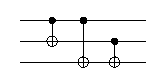
\includegraphics[scale=2]{Figures/circuits/bothEndsSimple}};  
      \node[above left=4.5mm and -7mm of circuit.west, opacity=0.9] {\footnotesize \(A\)};
      \node[left=-7mm of circuit.west, opacity=0.9] {\footnotesize \(B\)};
      \node[below left=4.5mm and -7mm of circuit.west, opacity=0.9] {\footnotesize \(C\)};
      \node[above right=0.8mm and 12.8mm of circuit.west, opacity=0.9] {\footnotesize \(\gamma\)};
      \node[below right=0.8mm and 23.6mm of circuit.west, opacity=0.9] {\footnotesize \(\beta\)};
      \node[below right=0.8mm and 34.4mm of circuit.west, opacity=0.9] {\footnotesize \(\alpha\)};
      \node[right=-3mm of circuit.north west, font=\itshape] (text) {a)};
    \end{tikzpicture}
  };
  \node[below=5mm of orig] (case1) {
    \begin{tikzpicture}
      \node[inner sep=0pt] (circuit) {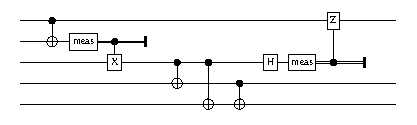
\includegraphics[scale=2]{Figures/circuits/bothEndsSimple1}};  
      \node[above left=4.5mm and -7mm of circuit.west, opacity=0.9] {\footnotesize \(A\)};
      \node[left=-7mm of circuit.west, opacity=0.9] {\footnotesize \(B\)};
      \node[below left=4.5mm and -7mm of circuit.west, opacity=0.9] {\footnotesize \(C\)};
      \node[above right=0.8mm and 12.8mm of circuit.west, opacity=0.9] {\footnotesize \(\gamma\)};
      \node[below right=0.8mm and 23.6mm of circuit.west, opacity=0.9] {\footnotesize \(\beta\)};
      \node[below right=0.8mm and 34.4mm of circuit.west, opacity=0.9] {\footnotesize \(\alpha\)};
      \node[right=-3mm of circuit.north west, font=\itshape] (text) {a)};
    \end{tikzpicture}
  };
  \node[below=5mm of case1] (case2) {
    \begin{tikzpicture}
      \node[inner sep=0pt] (circuit) {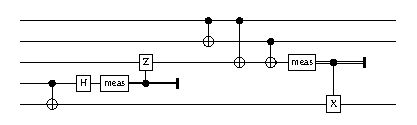
\includegraphics[scale=2]{Figures/circuits/bothEndsSimple2}};  
      \node[above left=4.5mm and -7mm of circuit.west, opacity=0.9] {\footnotesize \(A\)};
      \node[left=-7mm of circuit.west, opacity=0.9] {\footnotesize \(B\)};
      \node[below left=4.5mm and -7mm of circuit.west, opacity=0.9] {\footnotesize \(C\)};
      \node[above right=0.8mm and 12.8mm of circuit.west, opacity=0.9] {\footnotesize \(\gamma\)};
      \node[below right=0.8mm and 23.6mm of circuit.west, opacity=0.9] {\footnotesize \(\beta\)};
      \node[below right=0.8mm and 34.4mm of circuit.west, opacity=0.9] {\footnotesize \(\alpha\)};
      \node[right=-3mm of circuit.north west, font=\itshape] (text) {a)};
    \end{tikzpicture}
  };
\end{tikzpicture}
\caption{}
\label{fig:BothEndsSimple}
\end{figure}

\textbf{TODO}: Simply bothEndsSimple.pdf, distributed by common target and common control, discussing which CNOT becomes local.